\foreach \metric/\cap in \metrics{
    \begin{figure}[p]
        \centering
        \includegraphics[width=\textwidth]{chapters/experiments/img/merged_plots/main_snowball/\metric.png}
        \caption{\cap \space w zależności od liczby wierzchołków - próbkowanie snowball}
        \label{fig:main_snowball_\metric}
    \end{figure}
}

\newpage

\foreach \metric/\cap in \metrics{
    \begin{figure}[p]
        \centering
        \includegraphics[width=\textwidth]{chapters/experiments/img/merged_plots/main_twophase/\metric.png}
        \caption{\cap \space w zależności od liczby wierzchołków - próbkowanie dwufazowe}
        \label{fig:main_twophase_\metric}
    \end{figure}
}

\begin{figure}[h!]
    \centering
    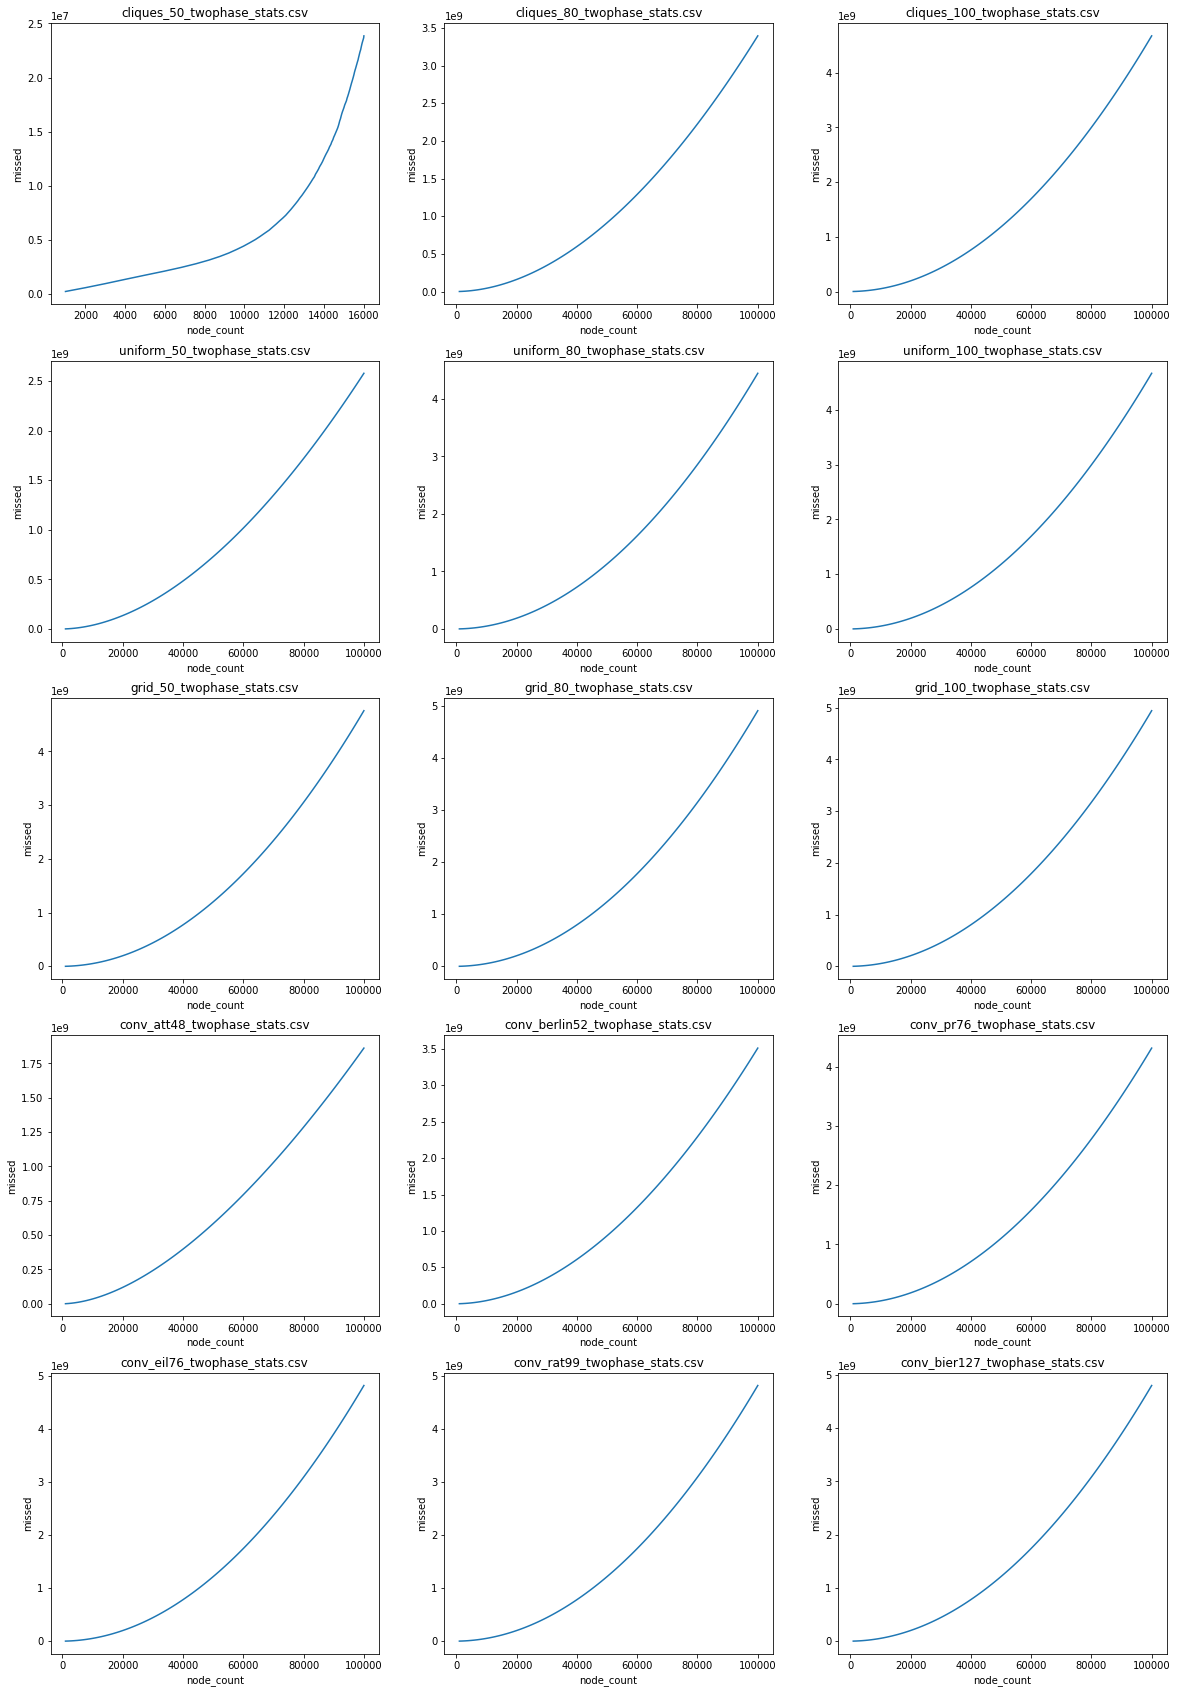
\includegraphics[width=\textwidth]{chapters/experiments/img/merged_plots/main_twophase/missed.png}
    \caption{Liczba nieudanych prób tworzenia krawędzi w zależności od liczby wierzchołków - próbkowanie dwufazowe}
    \label{fig:main_twophase_missed}
\end{figure}

\begin{figure}[h!]
    \centering
    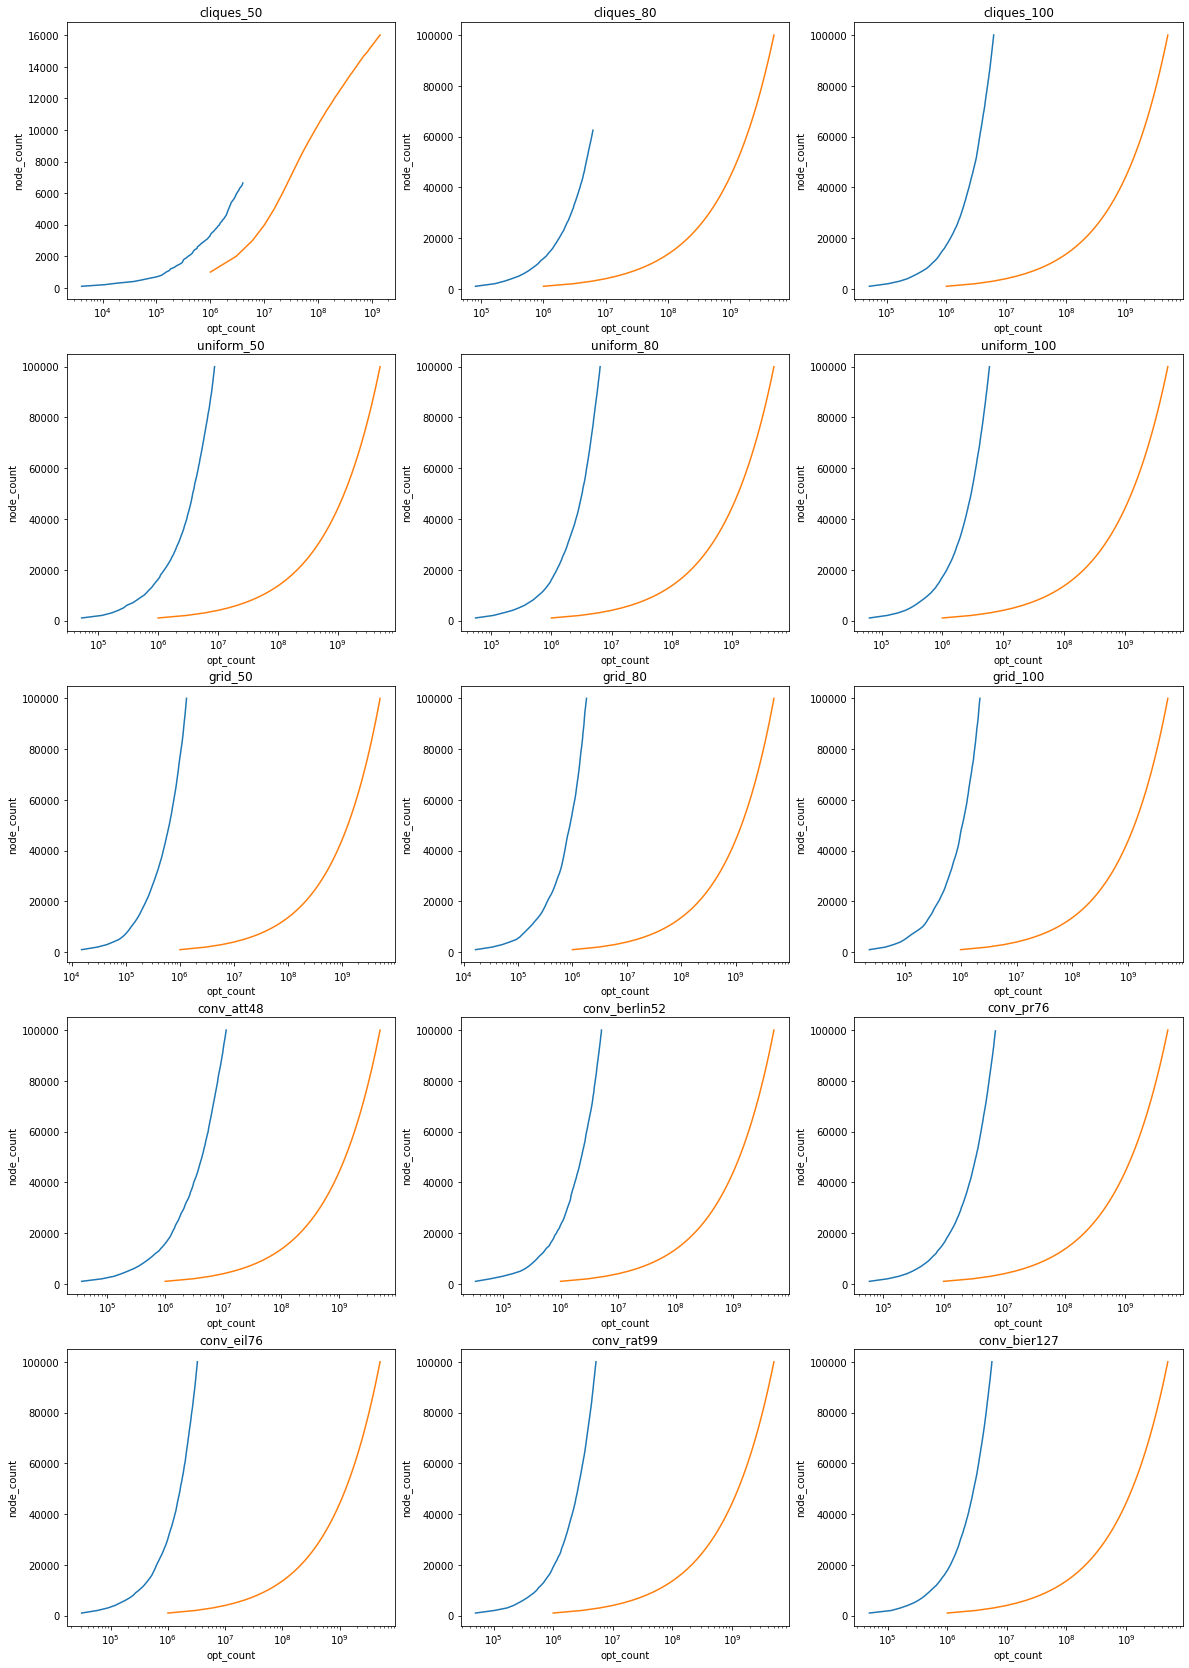
\includegraphics[width=\textwidth]{chapters/experiments/img/opt_nodes.png}
    \caption{Wykres zależności liczby wierzchołków od liczby wywołań funkcji celu.
        Kolor niebieski - próbkowanie snowball, kolor pomarańczowy - próbkowanie dwufazowe.
        Oś X w skali logarytmicznej}
    \label{fig:main_opt_nodes}
\end{figure}

\begin{figure}[h!]
    \centering
    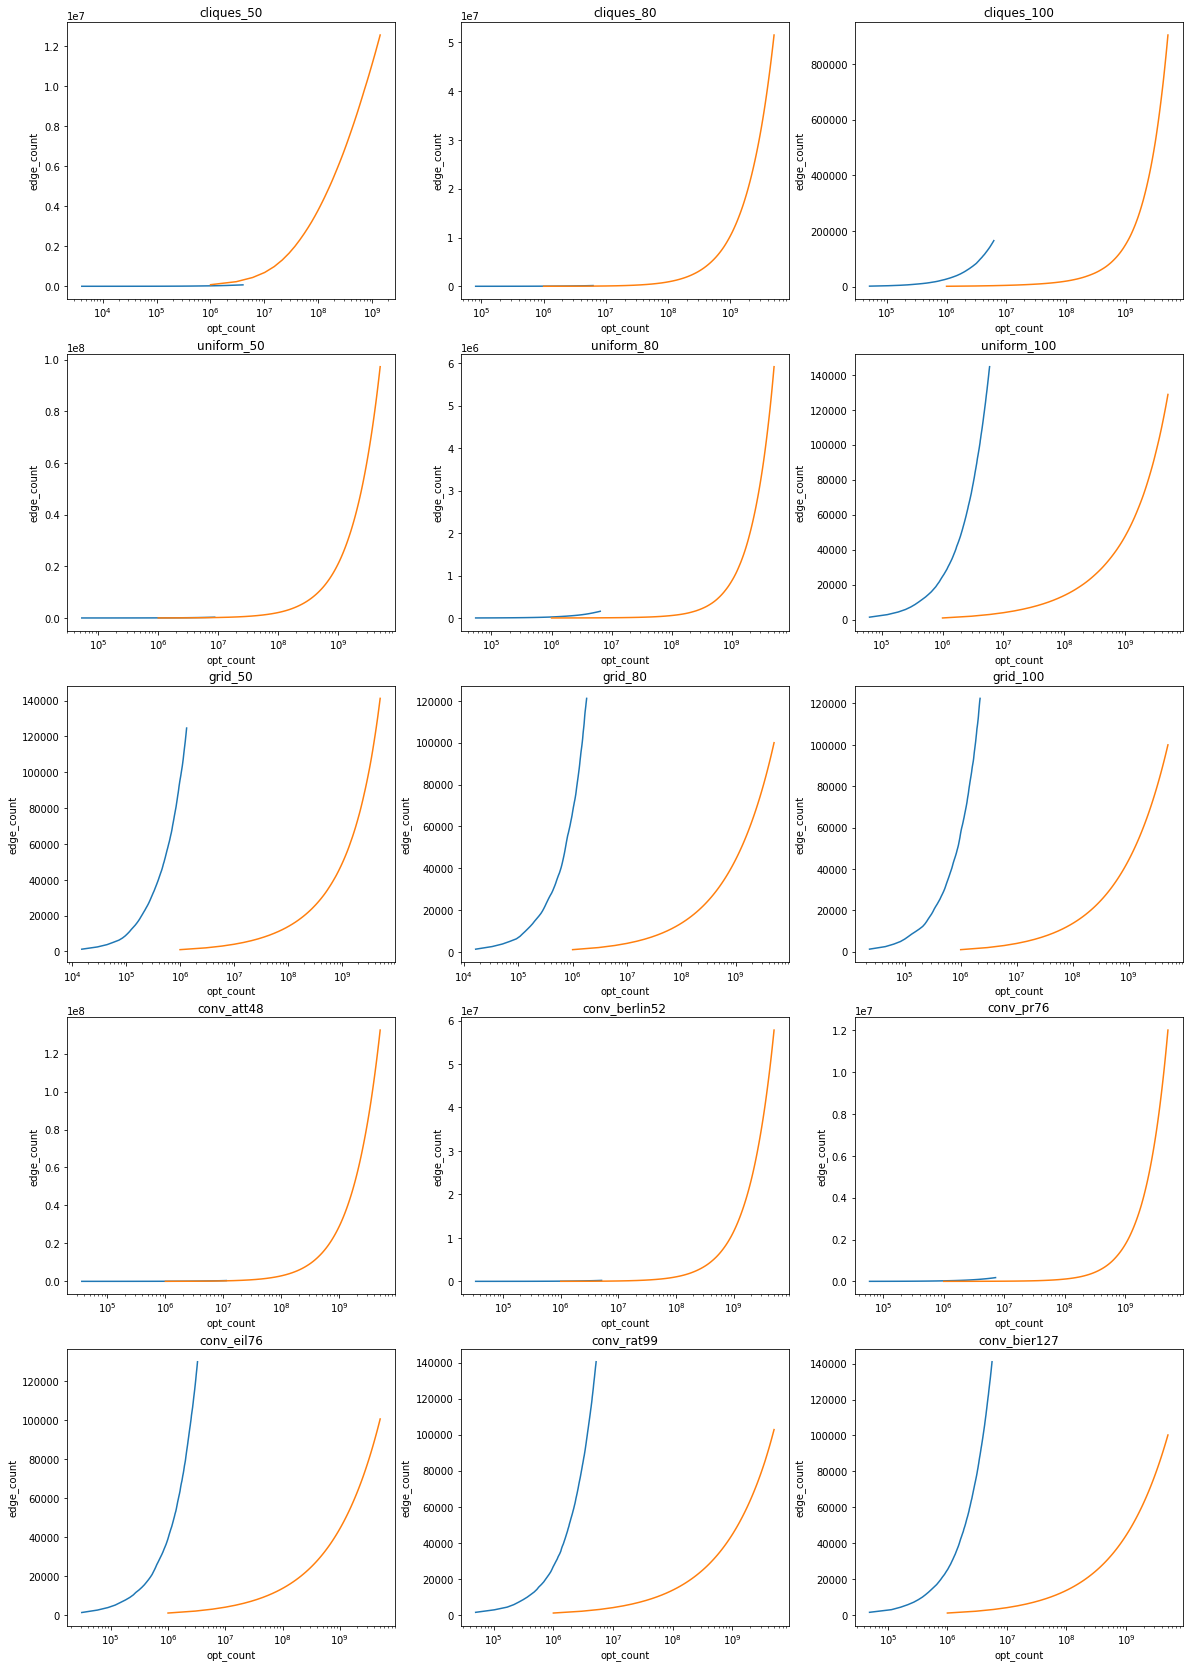
\includegraphics[width=\textwidth]{chapters/experiments/img/opt_edges.png}
    \caption{Wykres zależności liczby krawędzi od liczby wywołań funkcji celu.
        Kolor niebieski - próbkowanie snowball, kolor pomarańczowy - próbkowanie dwufazowe.
        Oś X w skali logarytmicznej}
    \label{fig:main_opt_edges}
\end{figure}


